% !TeX encoding=unicode
% !TeX spellcheck = de-DE

\chapter{Results}
%
\section{Grid validiation}
In the following we will validate the interpolation method used by \mcgrid{} for the processes $pp \rightarrow H + (0,1,2) \text{jets}$ at the \SI{13}{\tera\electronvolt} LHC, computed at NLO.
Thereto, we generate reference distributions for different observables using the \sherpa{} event generator and compare them to the distributions obtained by convoluting a grid with the respective PDF.
When possible, the results from \appl{} and \fnlo{} are compared to each other.
All grids are filled using the central value of the CT10 pdf set \cite{ct10}.
The examined observables are the transverse momenta $p_\perp$ of the Higgs boson and the $\tau$ leptons, respectively, the rapidity $y$ of the Higgs boson and the pseudorapidity $\eta$ of the $\tau$ leptons.
The projection of the observables into histogram bins is accomplished by the \rivet{} analysis system.
Final state jets are extracted by the \fastjet{} library \cite{fastjet_manual} using the anti-$k_t$ algorithm \cite{anti_kt} with a radius parameter $R=0.4$ and a $p_\perp$-cut of $p_\perp > \SI{20}{\giga\electronvolt}$.

The first validity test will check whether the grids are able to reproduce the distributions when they are filled with the same events as the reference histograms, i.e.\ when no parameter variation is performed.
This will also determine the interpolation accuracy.
Subsequently, the cases where the scale factors and/or PDFs of the grids are changed \textit{a posteriori} will be compared to reference distributions where these parameters have been set explicitly.
%
\subsection{Interpolation accuracy}
In this section we will prove, that the grids are able to reproduce the reference distributions up to the available interpolation accuracy.
For each observable, two grids are produced: One high precision grid with \num{50} bins in $x$ and \num{30} bins in $Q^2$ and one lower precision grid with \num{30} bins in $x$ and \textcolor{red}{???} bins in $Q^2$.
In the 0-jet case, only one $Q^2$ bin is used, because the scale parameters are fixed to the Higgs boson mass so that $Q^2$ does not change.
To achieve better comparability, \appl{} is configured to use fourth order interpolation, which is the same as is hardcoded into the \fnlo{} library.
A sample of \num{10} million events is used to fill the grids.

\Cref{fig:hnlo_validation} shows the ratio of the results obtained by convoluting the grids with the CT10 PDF to the reference distributions.
In all cases, the reproduction accuracy is well below \SI{1}{\percent} and for most of the bins it is even better than \SI{0.1}{\percent}.
The $p_\perp$ distributions produced by \appl{} are much more sensitive to the grid size than the ones produced by \fnlo{}.
For the rapidity distributions, the differnce between the high and the low precision grid is negligible
%
\begin{sidewaysfigure}
\centering
\begin{subfigure}[]{0.49\textwidth}
	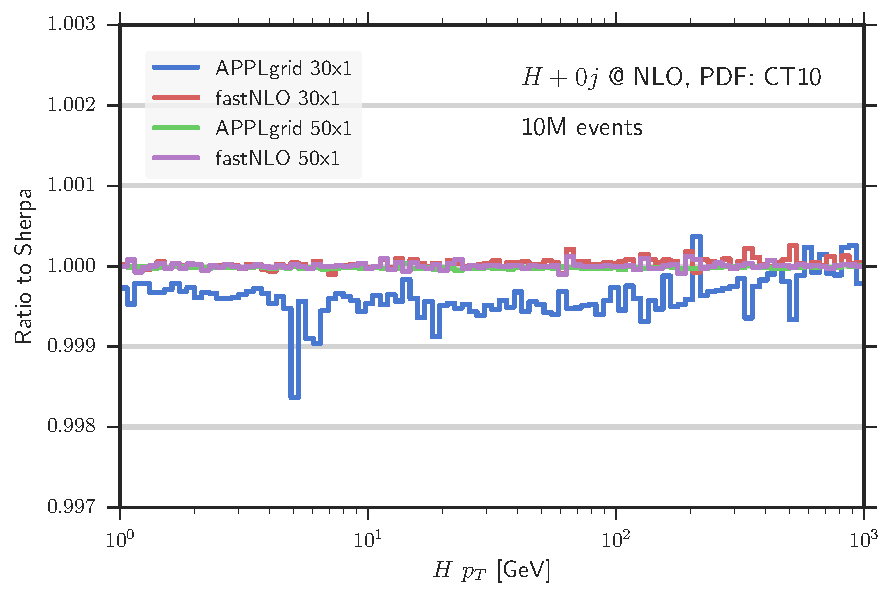
\includegraphics[width=\textwidth]{images/hnlo_hpt_50v30.pdf}
\end{subfigure}
\hfill
\begin{subfigure}[]{0.49\textwidth}
	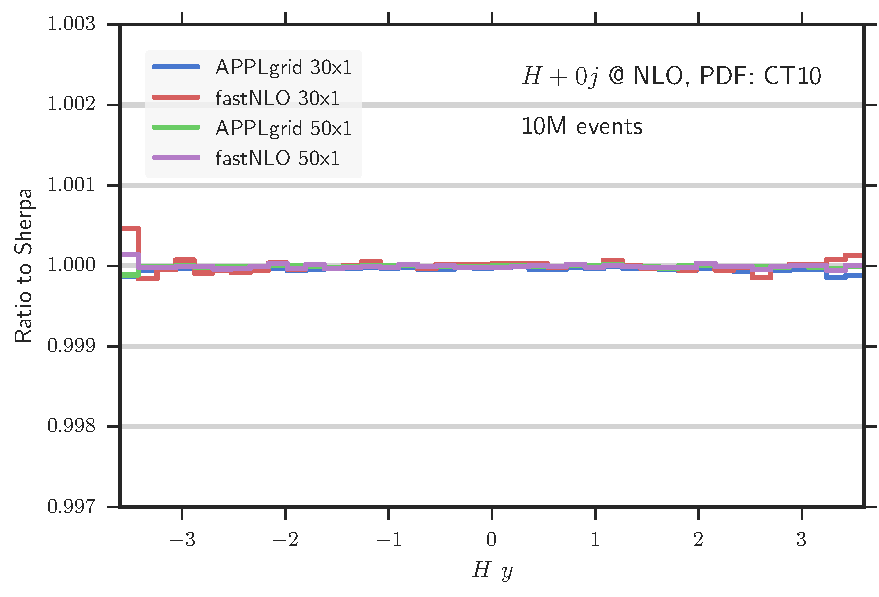
\includegraphics[width=\textwidth]{images/hnlo_hy_50v30.pdf}
\end{subfigure}

\begin{subfigure}[]{0.49\textwidth}
	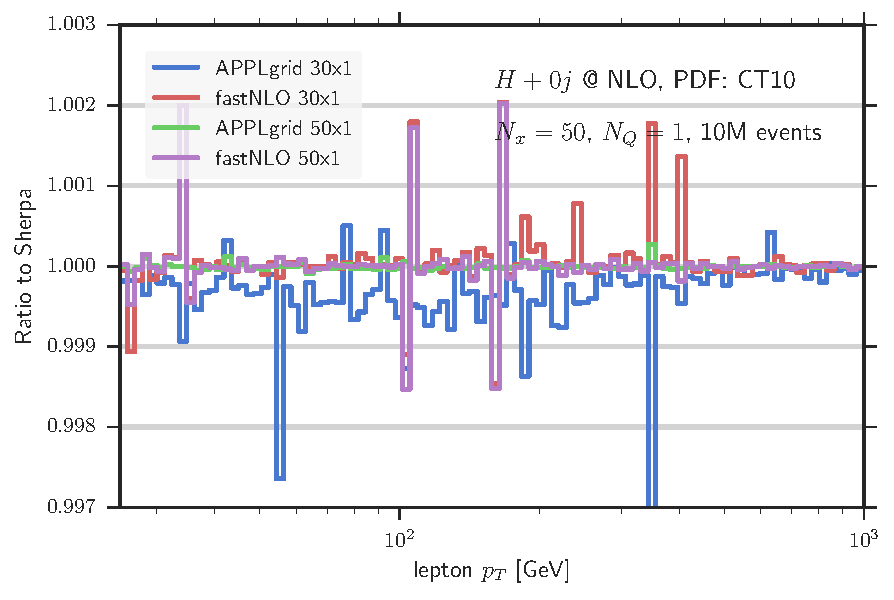
\includegraphics[width=\textwidth]{images/hnlo_lpt_50v30.pdf}
\end{subfigure}
\hfill
\begin{subfigure}[]{0.49\textwidth}
	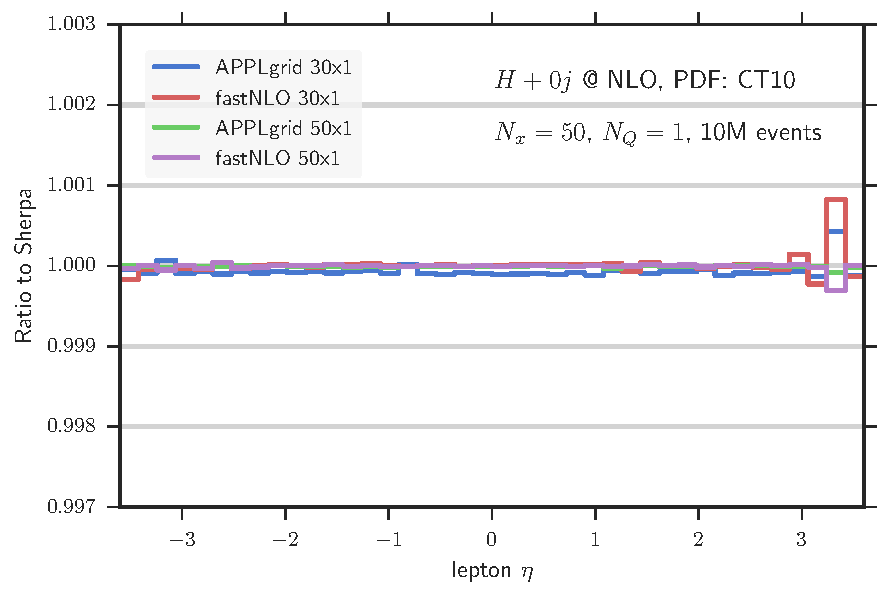
\includegraphics[width=\textwidth]{images/hnlo_leta_50v30.pdf}
\end{subfigure}
\caption{H+0j NLO}
\label{fig:hnlo_validation}
\end{sidewaysfigure}
%


%
\begin{figure}
%% No H pT at Born, lpt_max = m_H / 2
\centering
%\begin{subfigure}[]{0.49\textwidth}
%	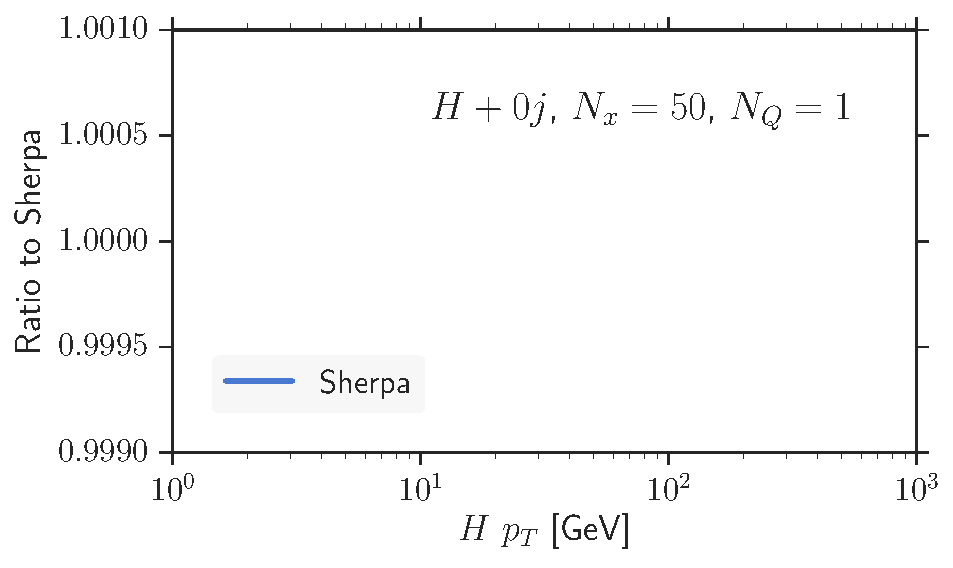
\includegraphics[width=\textwidth]{images/hb_hpt.pdf}
%\end{subfigure}
\hfill
\begin{subfigure}[]{0.49\textwidth}
	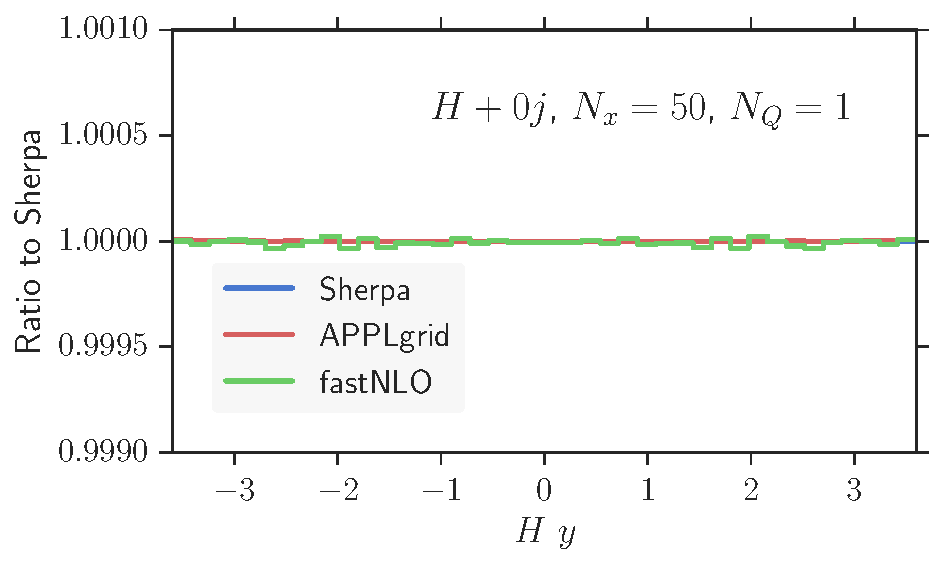
\includegraphics[width=\textwidth]{images/hb_hy.pdf}
\end{subfigure}

\begin{subfigure}[]{0.49\textwidth}
	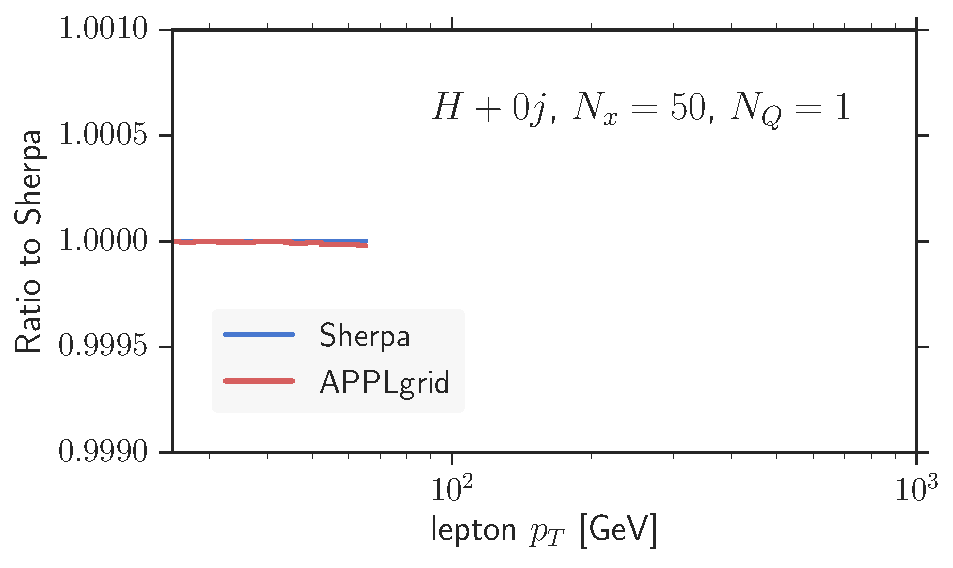
\includegraphics[width=\textwidth]{images/hb_lpt.pdf}
\end{subfigure}
\hfill
\begin{subfigure}[]{0.49\textwidth}
	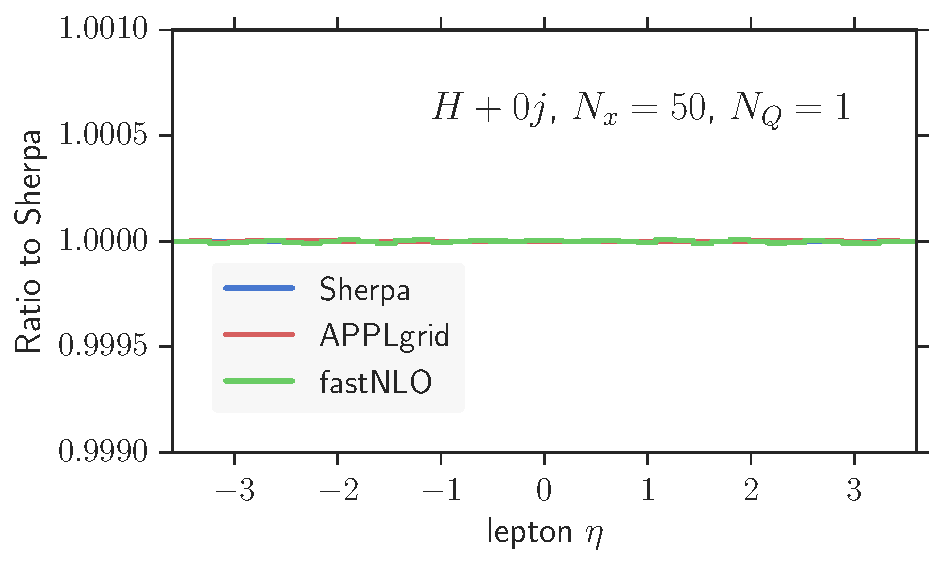
\includegraphics[width=\textwidth]{images/hb_leta.pdf}
\end{subfigure}
\caption{H B}
%\label{fig:bla}
\end{figure}
%
\begin{figure}
\centering
\begin{subfigure}[]{0.49\textwidth}
	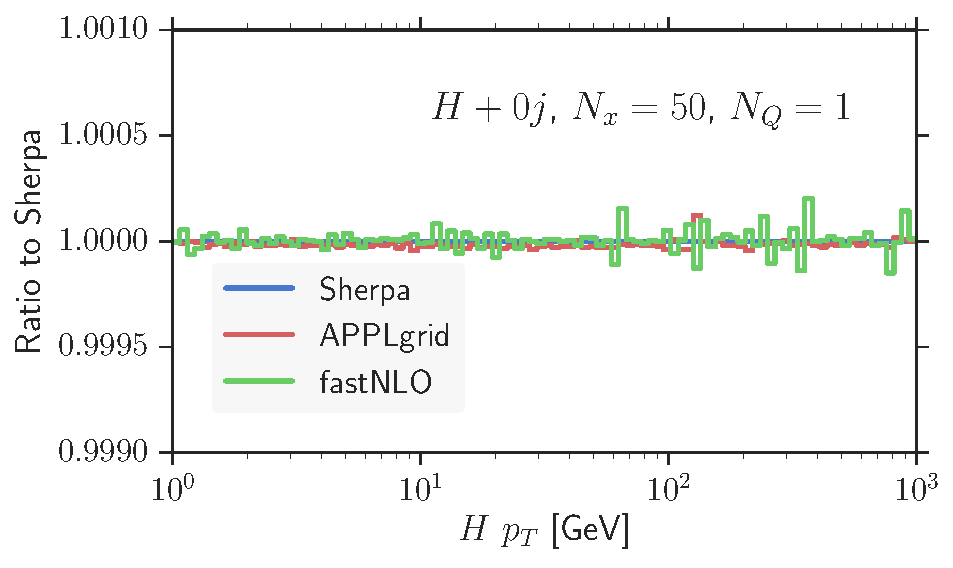
\includegraphics[width=\textwidth]{images/hrs_hpt.pdf}
\end{subfigure}
\hfill
\begin{subfigure}[]{0.49\textwidth}
	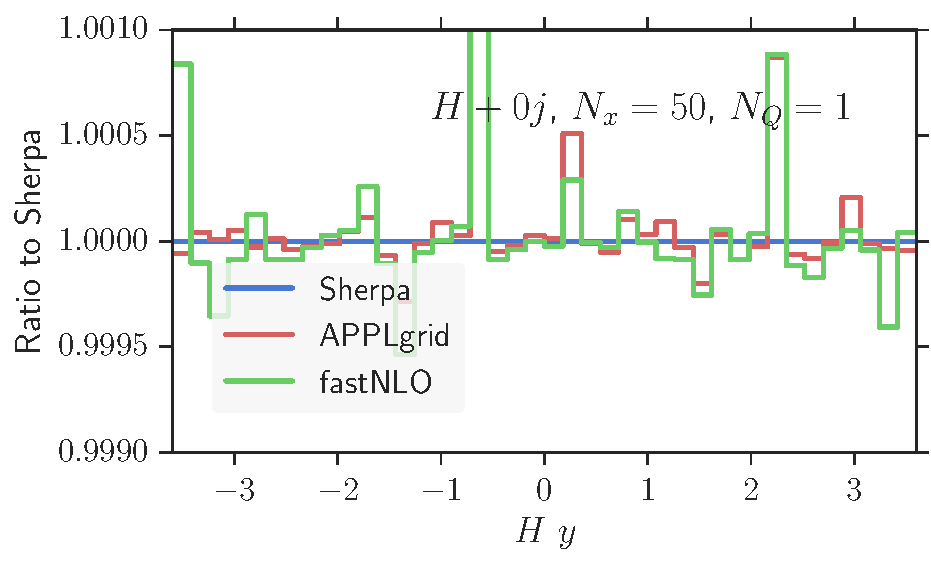
\includegraphics[width=\textwidth]{images/hrs_hy.pdf}
\end{subfigure}

\begin{subfigure}[]{0.49\textwidth}
	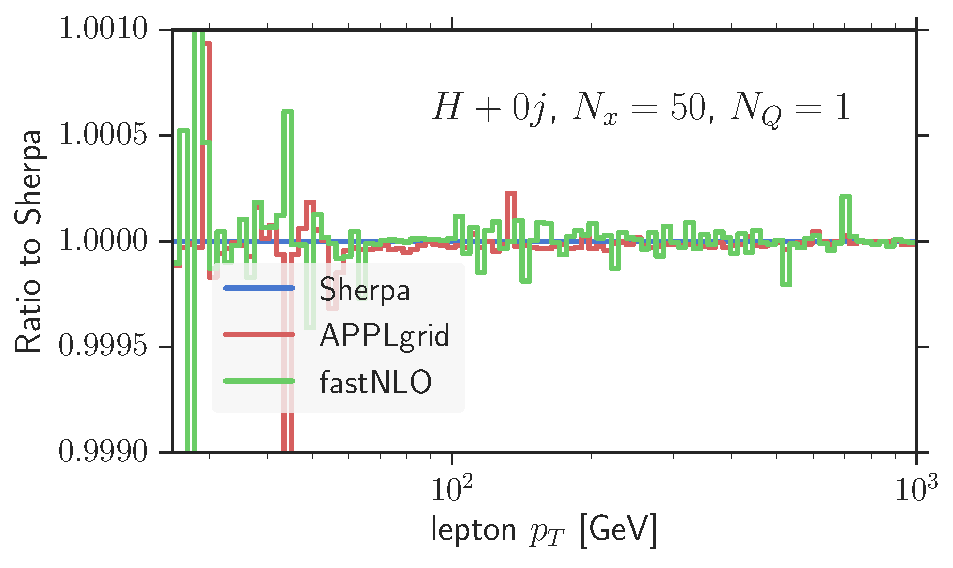
\includegraphics[width=\textwidth]{images/hrs_lpt.pdf}
\end{subfigure}
\hfill
\begin{subfigure}[]{0.49\textwidth}
	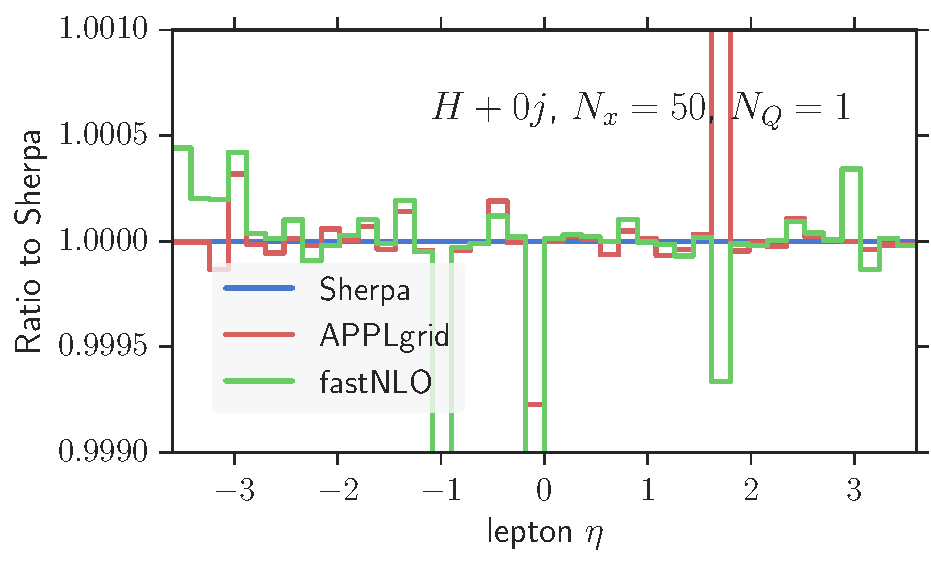
\includegraphics[width=\textwidth]{images/hrs_leta.pdf}
\end{subfigure}
\caption{H RS}
%\label{fig:bla}
\end{figure}
%
\begin{figure}
\centering
%\begin{subfigure}[]{0.49\textwidth}
%	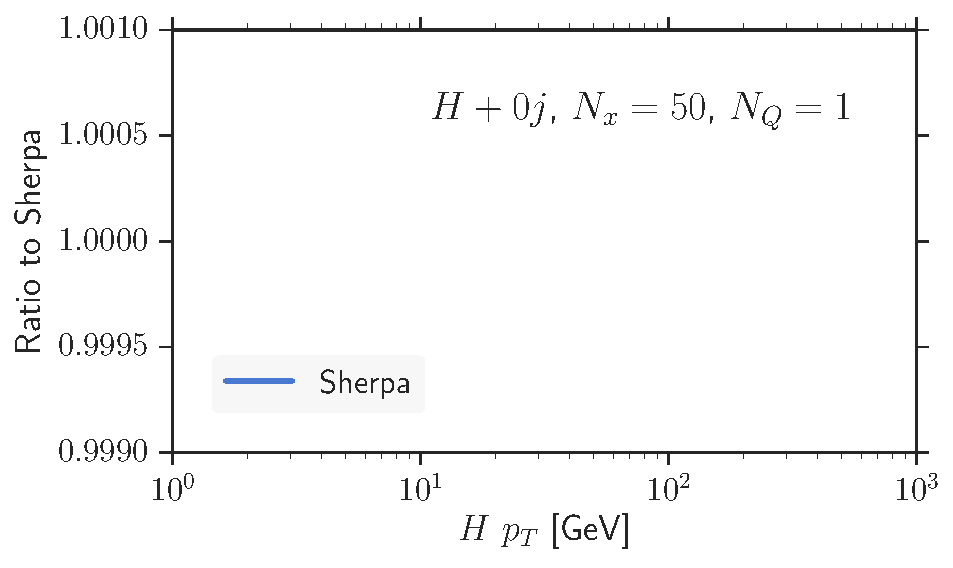
\includegraphics[width=\textwidth]{images/hvi_hpt.pdf}
%\end{subfigure}
\hfill
\begin{subfigure}[]{0.49\textwidth}
	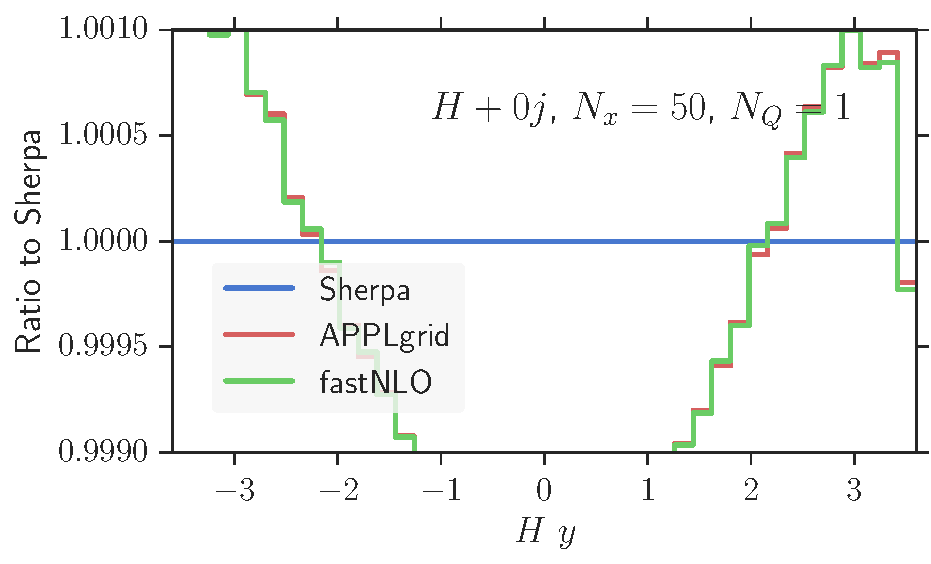
\includegraphics[width=\textwidth]{images/hvi_hy.pdf}
\end{subfigure}

\begin{subfigure}[]{0.49\textwidth}
	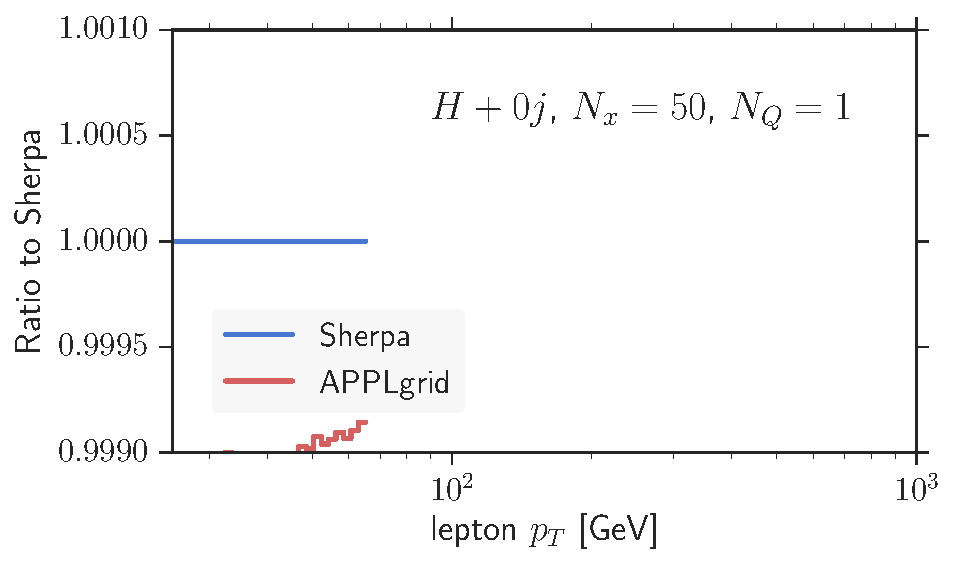
\includegraphics[width=\textwidth]{images/hvi_lpt.pdf}
\end{subfigure}
\hfill
\begin{subfigure}[]{0.49\textwidth}
	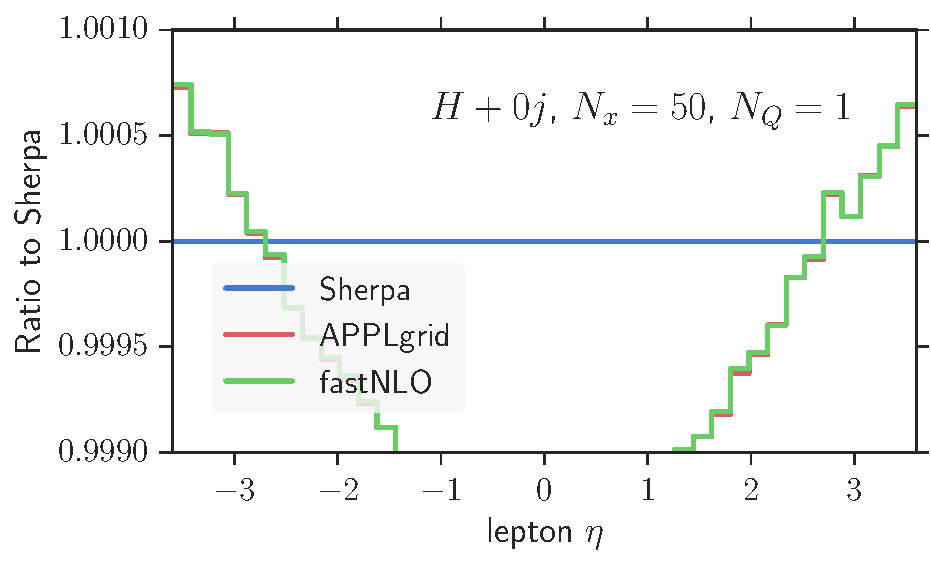
\includegraphics[width=\textwidth]{images/hvi_leta.pdf}
\end{subfigure}
\caption{H VI}
%\label{fig:bla}
\end{figure}
%
\begin{figure}
\centering
\begin{subfigure}[]{0.49\textwidth}
	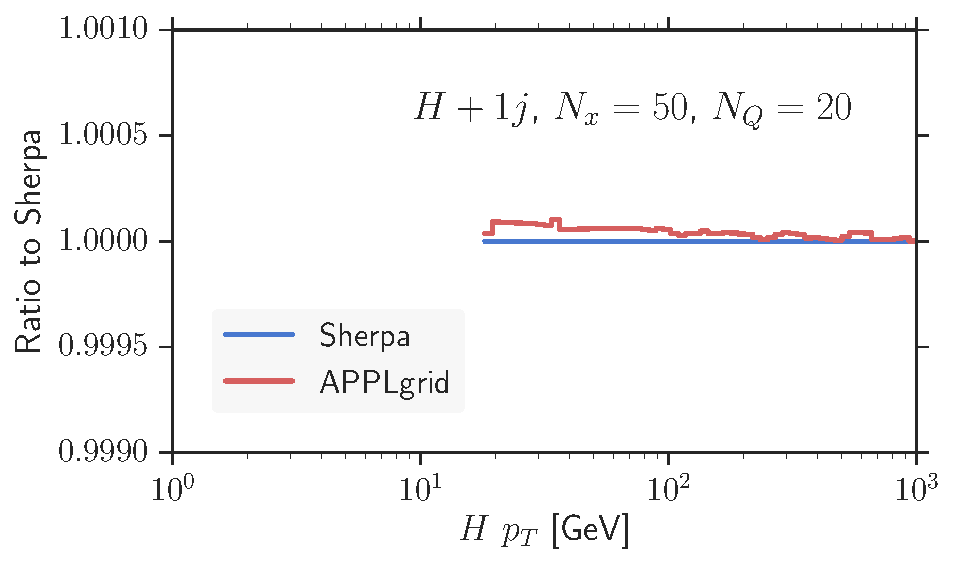
\includegraphics[width=\textwidth]{images/hjb_hpt.pdf}
\end{subfigure}
\hfill
\begin{subfigure}[]{0.49\textwidth}
	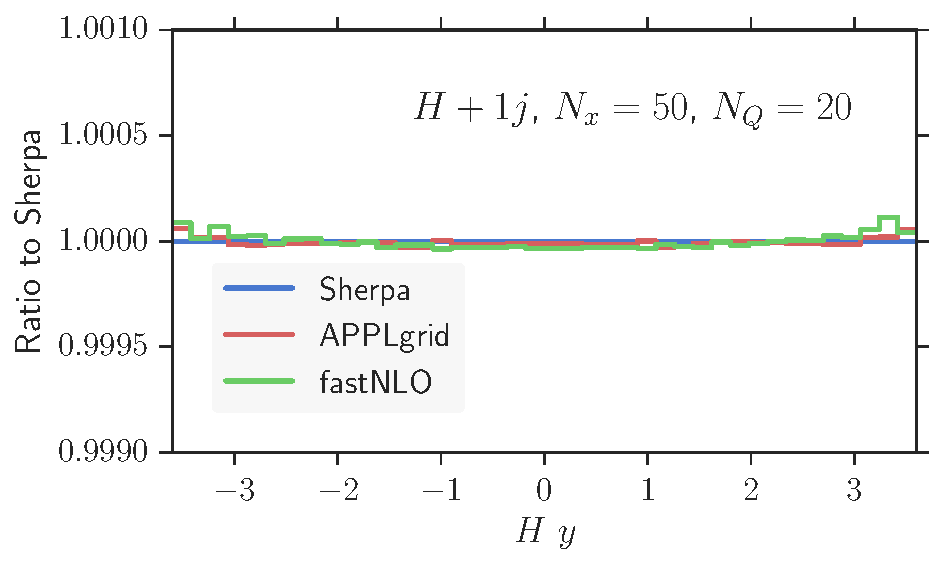
\includegraphics[width=\textwidth]{images/hjb_hy.pdf}
\end{subfigure}

\begin{subfigure}[]{0.49\textwidth}
	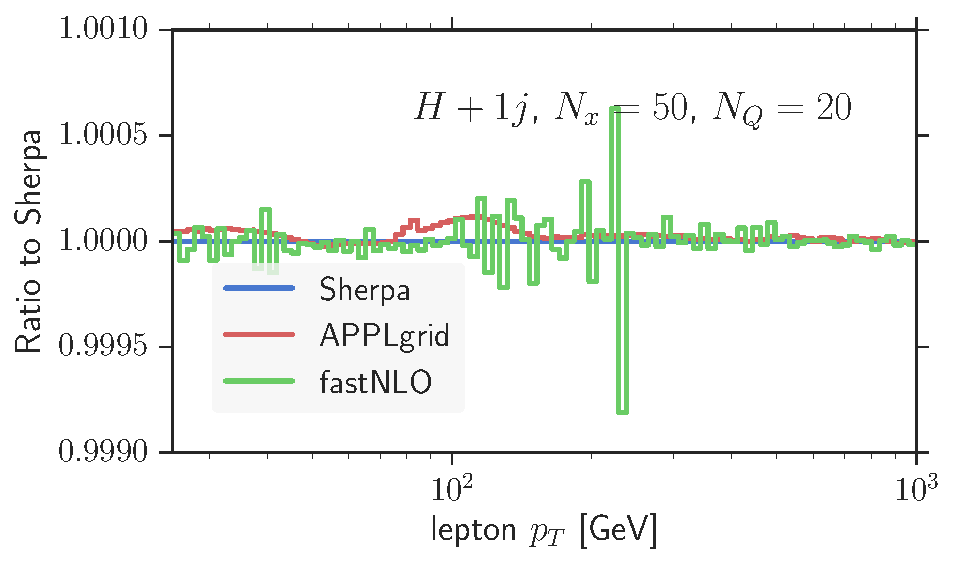
\includegraphics[width=\textwidth]{images/hjb_lpt.pdf}
\end{subfigure}
\hfill
\begin{subfigure}[]{0.49\textwidth}
	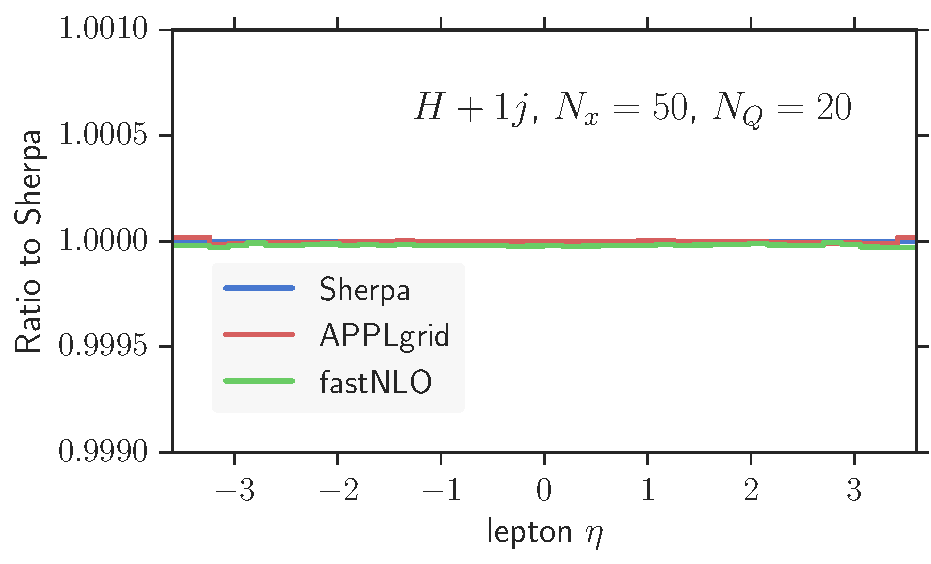
\includegraphics[width=\textwidth]{images/hjb_leta.pdf}
\end{subfigure}
\caption{Hj B}
%\label{fig:bla}
\end{figure}
%
\begin{figure}
\centering
\begin{subfigure}[]{0.49\textwidth}
	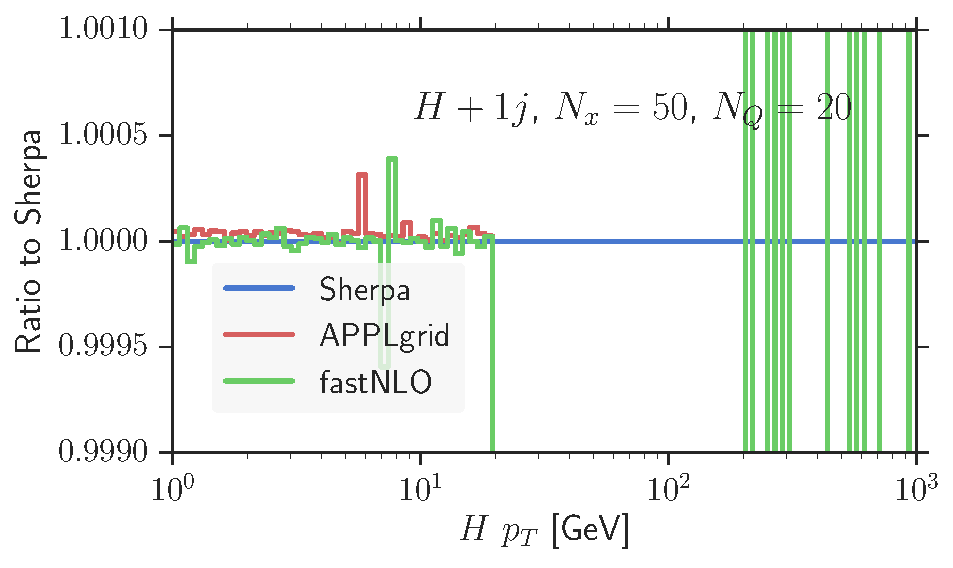
\includegraphics[width=\textwidth]{images/hjrs_hpt.pdf}
\end{subfigure}
\hfill
\begin{subfigure}[]{0.49\textwidth}
	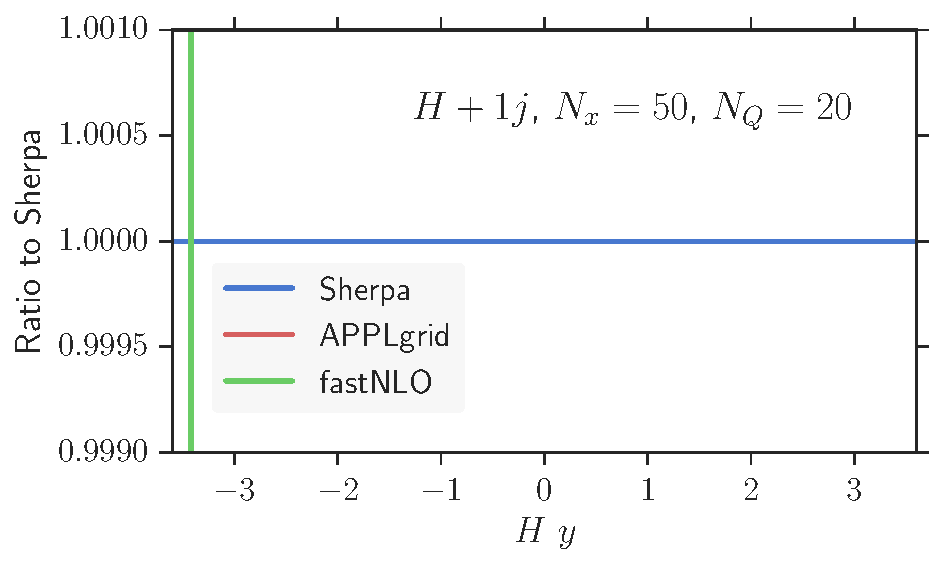
\includegraphics[width=\textwidth]{images/hjrs_hy.pdf}
\end{subfigure}

\begin{subfigure}[]{0.49\textwidth}
	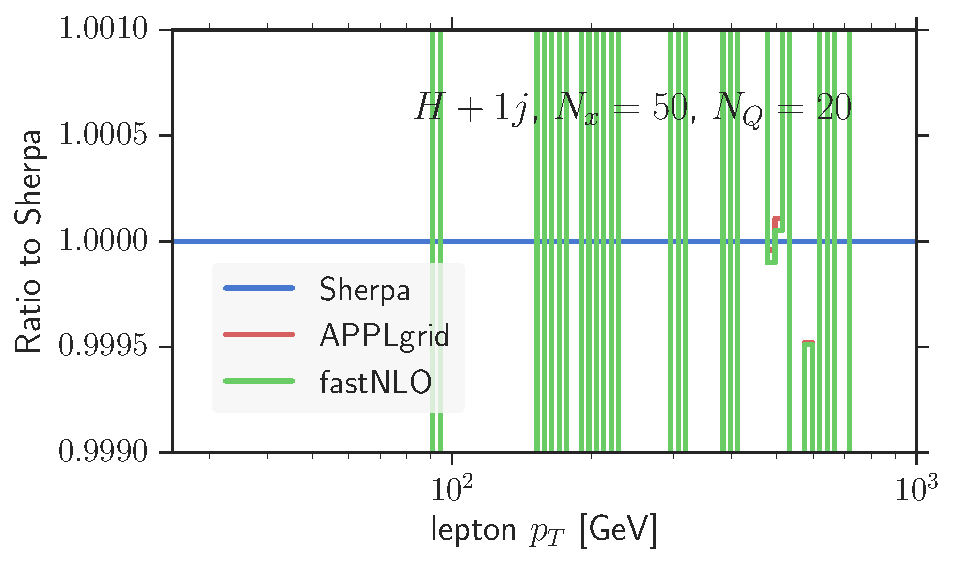
\includegraphics[width=\textwidth]{images/hjrs_lpt.pdf}
\end{subfigure}
\hfill
\begin{subfigure}[]{0.49\textwidth}
	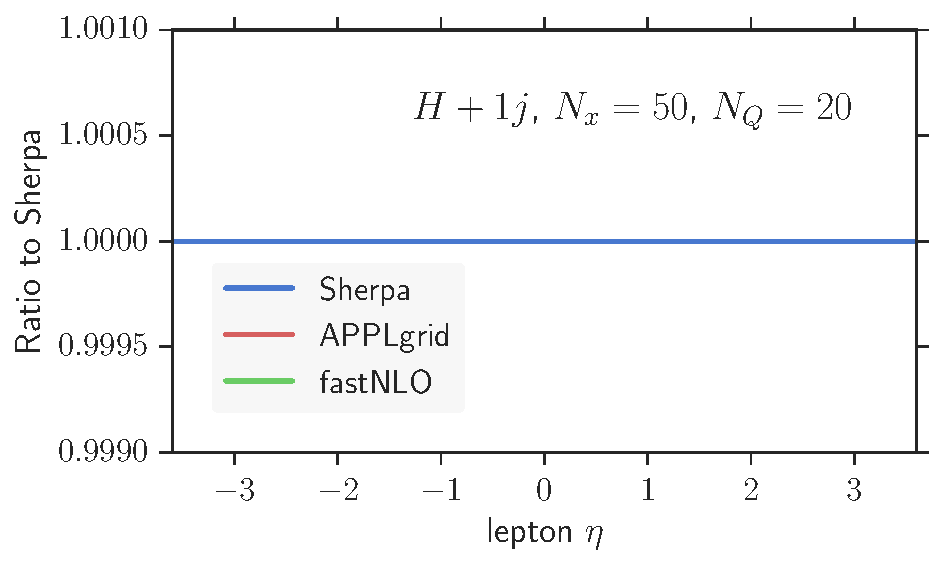
\includegraphics[width=\textwidth]{images/hjrs_leta.pdf}
\end{subfigure}
\caption{Hj RS}
%\label{fig:bla}
\end{figure}
%
\begin{figure}
\centering
\begin{subfigure}[]{0.49\textwidth}
	%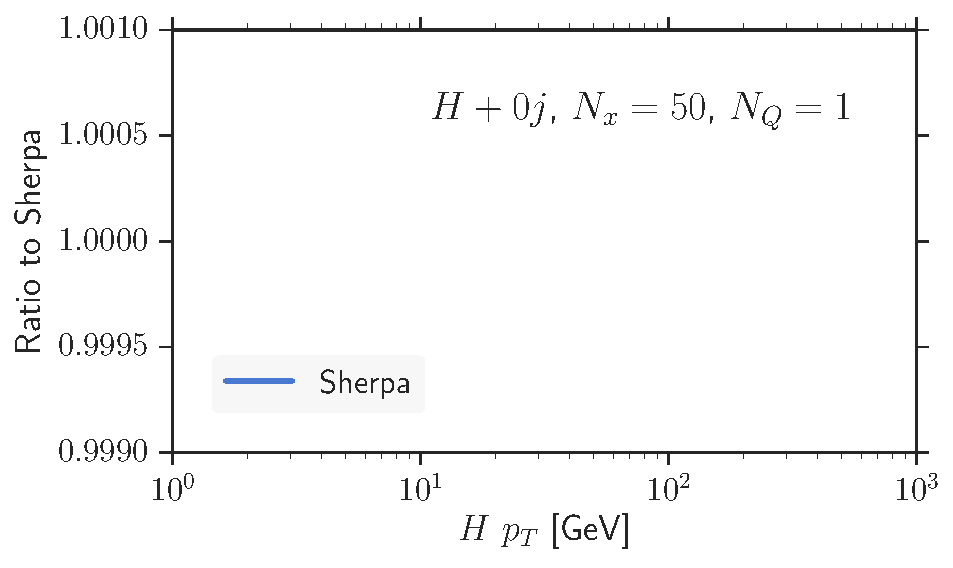
\includegraphics[width=\textwidth]{images/hb_hpt.pdf}
	
\includegraphics[width=\textwidth]{images/dummy.pdf}
\end{subfigure}
\hfill
\begin{subfigure}[]{0.49\textwidth}
	%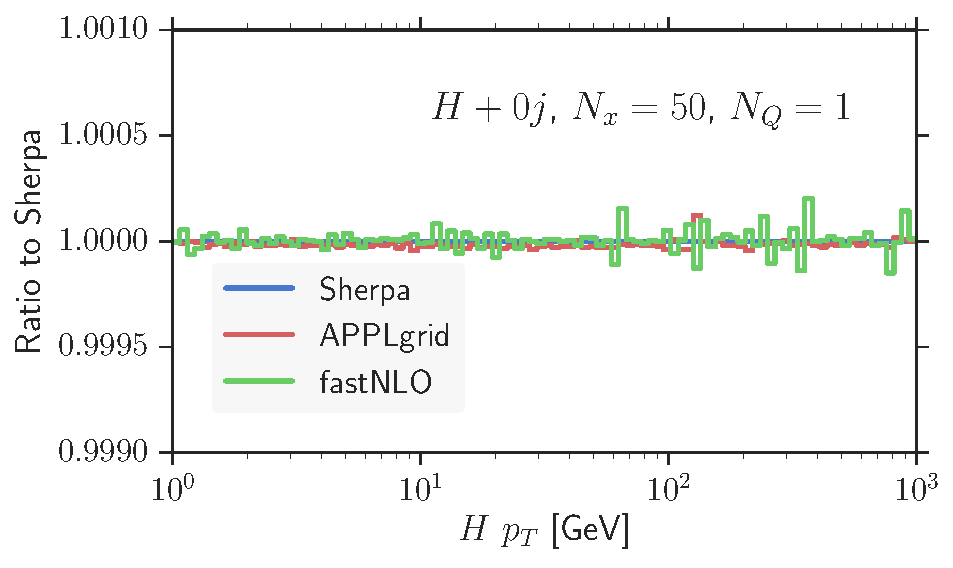
\includegraphics[width=\textwidth]{images/hrs_hpt.pdf}
	
\includegraphics[width=\textwidth]{images/dummy.pdf}
\end{subfigure}

\begin{subfigure}[]{0.49\textwidth}
	%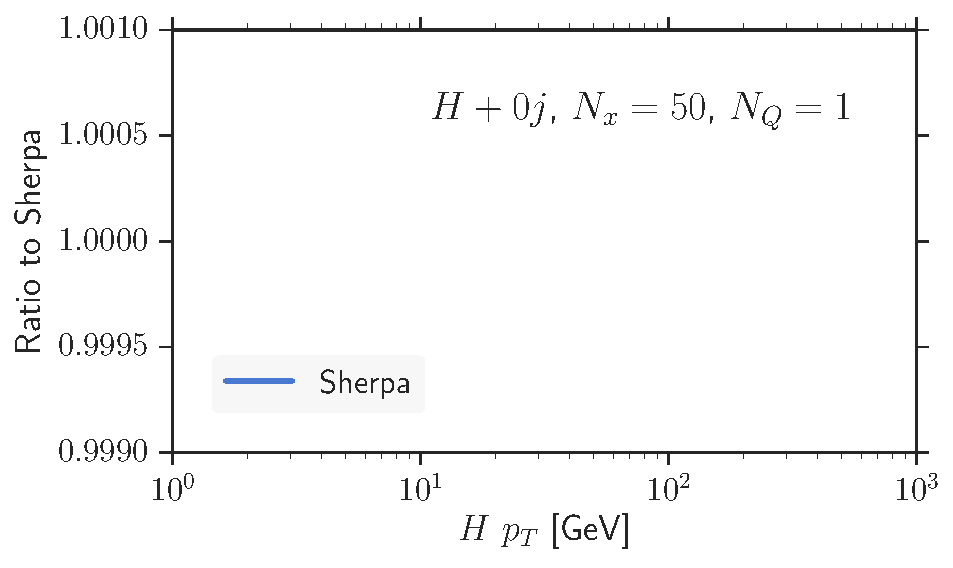
\includegraphics[width=\textwidth]{images/hvi_hpt.pdf}
	
\includegraphics[width=\textwidth]{images/dummy.pdf}
\end{subfigure}
\hfill
\begin{subfigure}[]{0.49\textwidth}
	%\includegraphics[width=\textwidth]{images/hb_hptpeak.pdf}
	
\includegraphics[width=\textwidth]{images/dummy.pdf}
\end{subfigure}
\caption{Hj VI}
%\label{fig:bla}
\end{figure}
%
\begin{figure}
\centering
\begin{subfigure}[]{0.49\textwidth}
	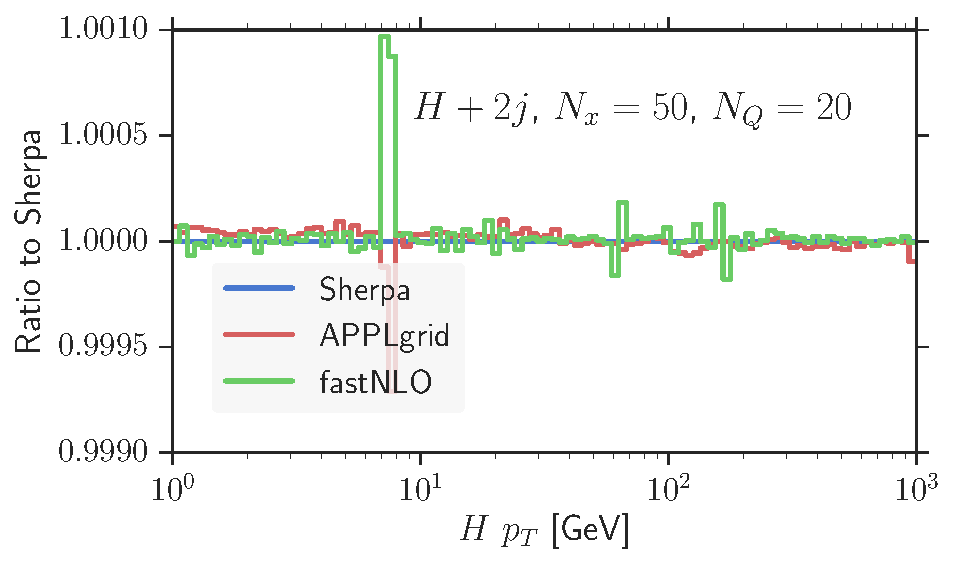
\includegraphics[width=\textwidth]{images/hjjb_hpt.pdf}
\end{subfigure}
\hfill
\begin{subfigure}[]{0.49\textwidth}
	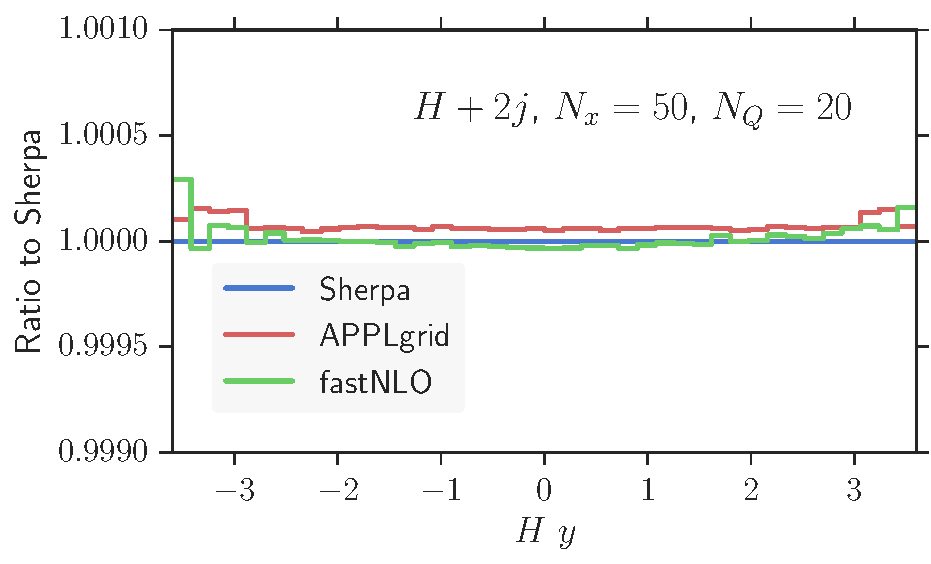
\includegraphics[width=\textwidth]{images/hjjb_hy.pdf}
\end{subfigure}

\begin{subfigure}[]{0.49\textwidth}
	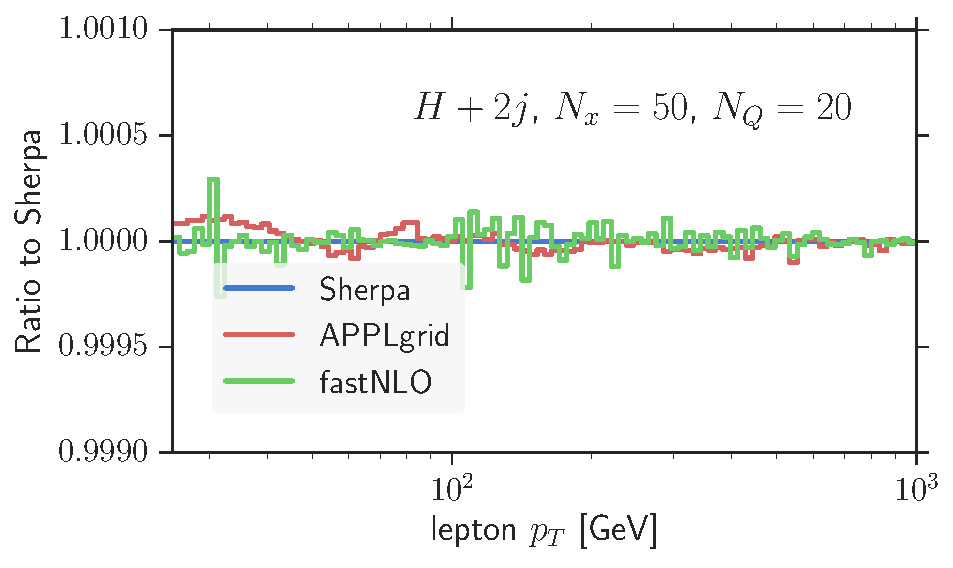
\includegraphics[width=\textwidth]{images/hjjb_lpt.pdf}
\end{subfigure}
\hfill
\begin{subfigure}[]{0.49\textwidth}
	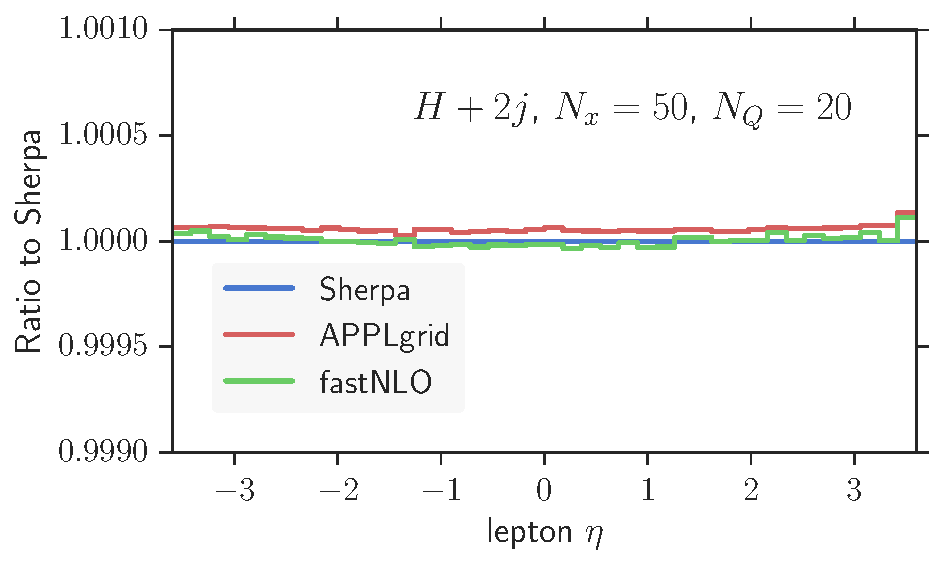
\includegraphics[width=\textwidth]{images/hjjb_leta.pdf}
\end{subfigure}
\caption{Hjj B}
%\label{fig:bla}
\end{figure}
%
\begin{figure}
\centering
\begin{subfigure}[]{0.49\textwidth}
	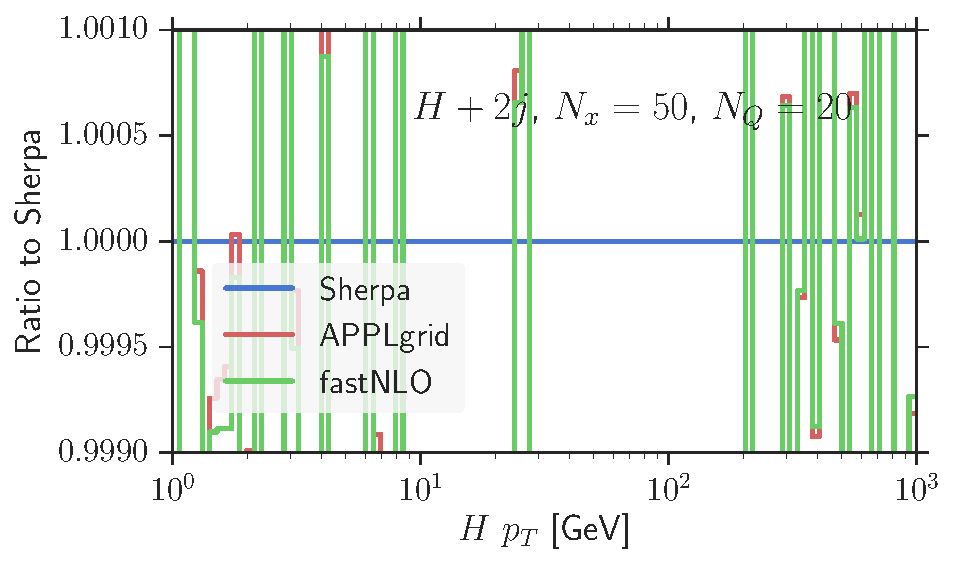
\includegraphics[width=\textwidth]{images/hjjrs_hpt.pdf}
\end{subfigure}
\hfill
\begin{subfigure}[]{0.49\textwidth}
	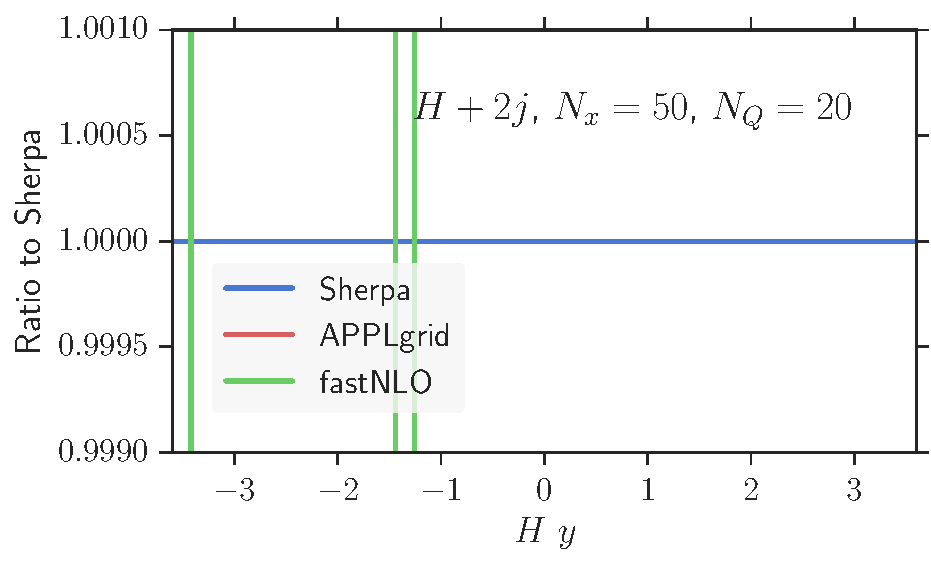
\includegraphics[width=\textwidth]{images/hjjrs_hy.pdf}
\end{subfigure}

\begin{subfigure}[]{0.49\textwidth}
	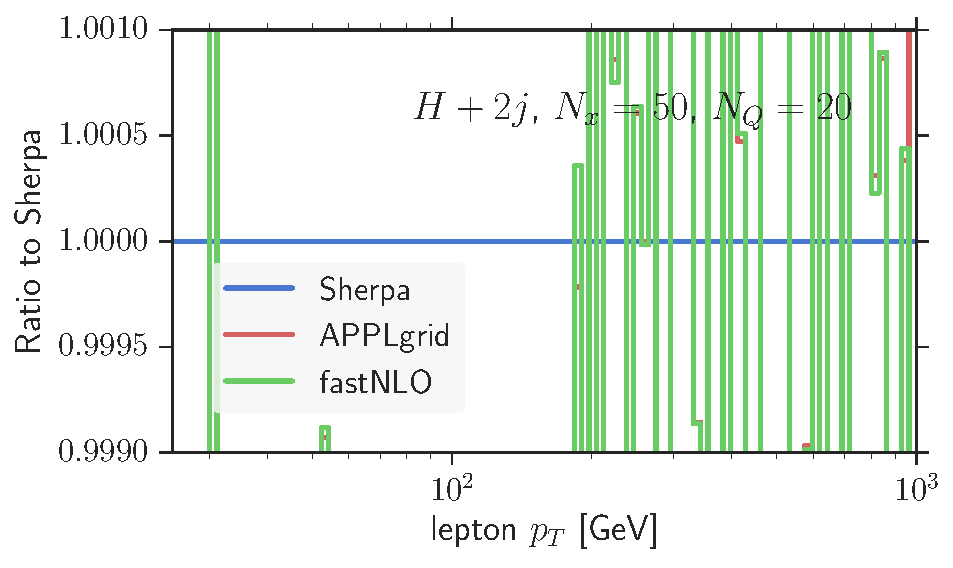
\includegraphics[width=\textwidth]{images/hjjrs_lpt.pdf}
\end{subfigure}
\hfill
\begin{subfigure}[]{0.49\textwidth}
	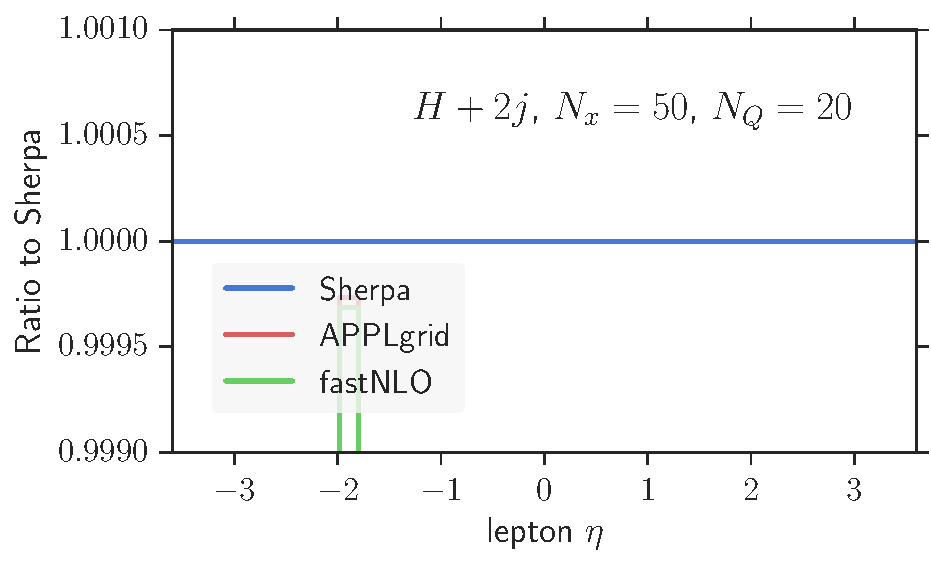
\includegraphics[width=\textwidth]{images/hjjrs_leta.pdf}
\end{subfigure}
\caption{Hjj RS}
%\label{fig:bla}
\end{figure}
%
\begin{figure}
\centering
\begin{subfigure}[]{0.49\textwidth}
	%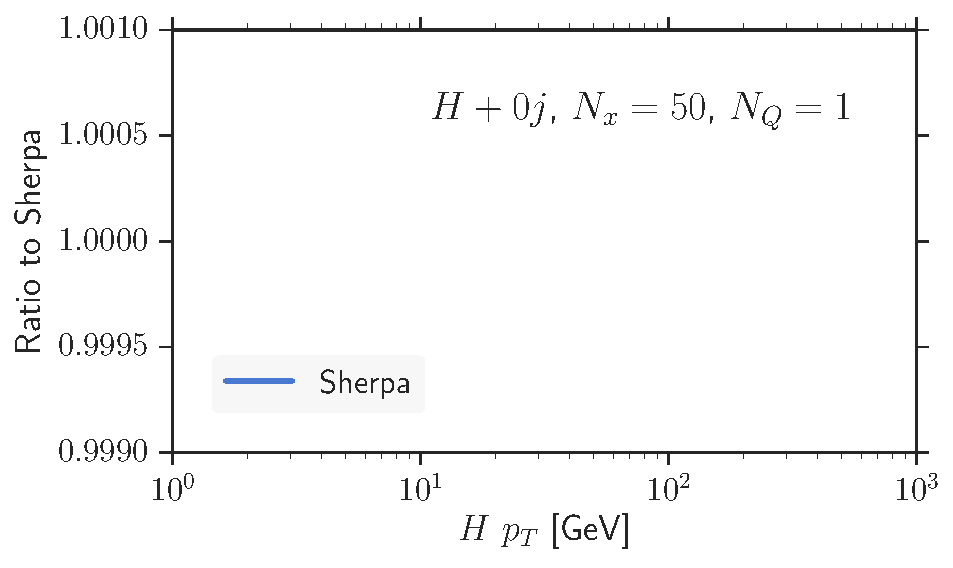
\includegraphics[width=\textwidth]{images/hb_hpt.pdf}
	
\includegraphics[width=\textwidth]{images/dummy.pdf}
\end{subfigure}
\hfill
\begin{subfigure}[]{0.49\textwidth}
	%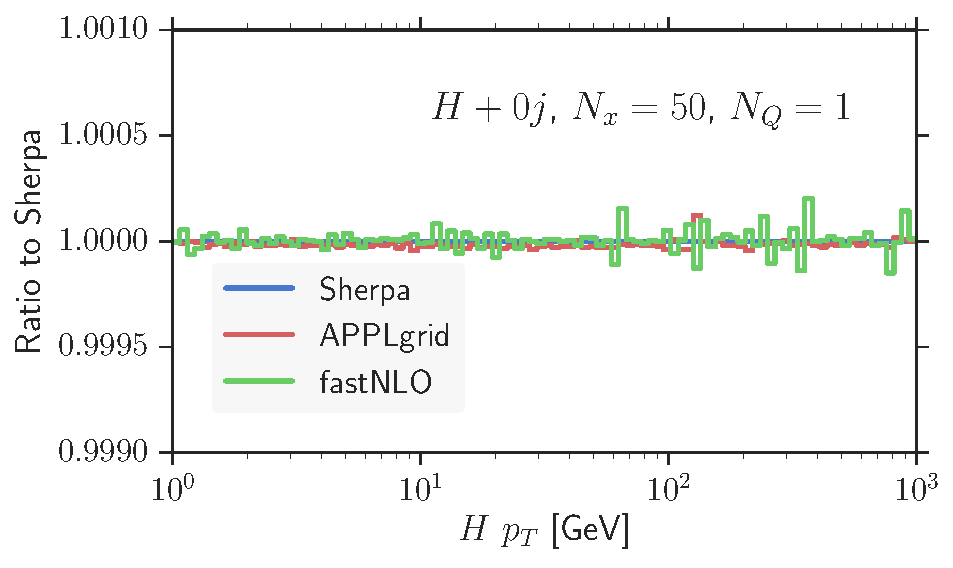
\includegraphics[width=\textwidth]{images/hrs_hpt.pdf}
	
\includegraphics[width=\textwidth]{images/dummy.pdf}
\end{subfigure}

\begin{subfigure}[]{0.49\textwidth}
	%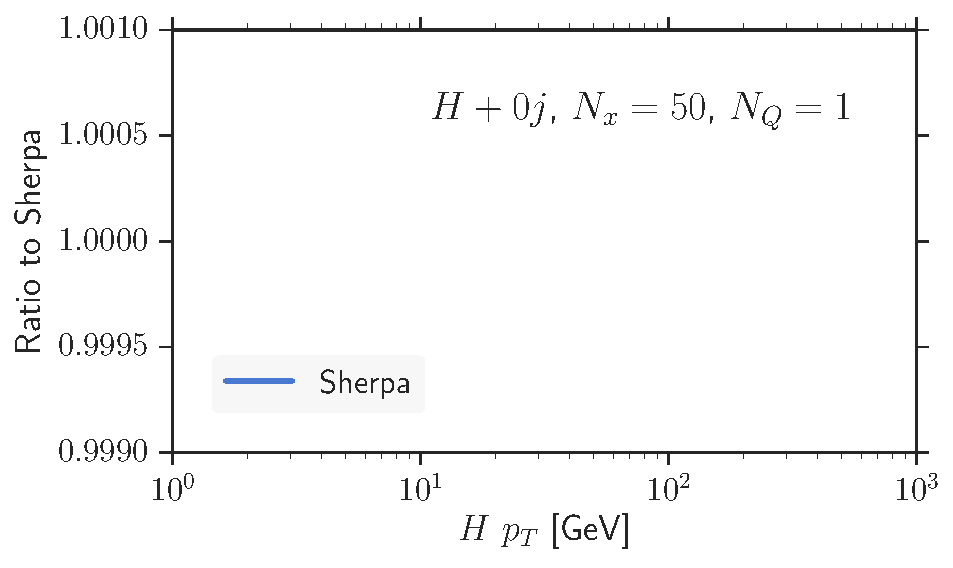
\includegraphics[width=\textwidth]{images/hvi_hpt.pdf}
	
\includegraphics[width=\textwidth]{images/dummy.pdf}
\end{subfigure}
\hfill
\begin{subfigure}[]{0.49\textwidth}
	%\includegraphics[width=\textwidth]{images/hb_hptpeak.pdf}
	
\includegraphics[width=\textwidth]{images/dummy.pdf}
\end{subfigure}
\caption{Hjj VI}
%\label{fig:bla}
\end{figure}
%



%
\begin{figure}
\centering
\begin{subfigure}[]{0.49\textwidth}
	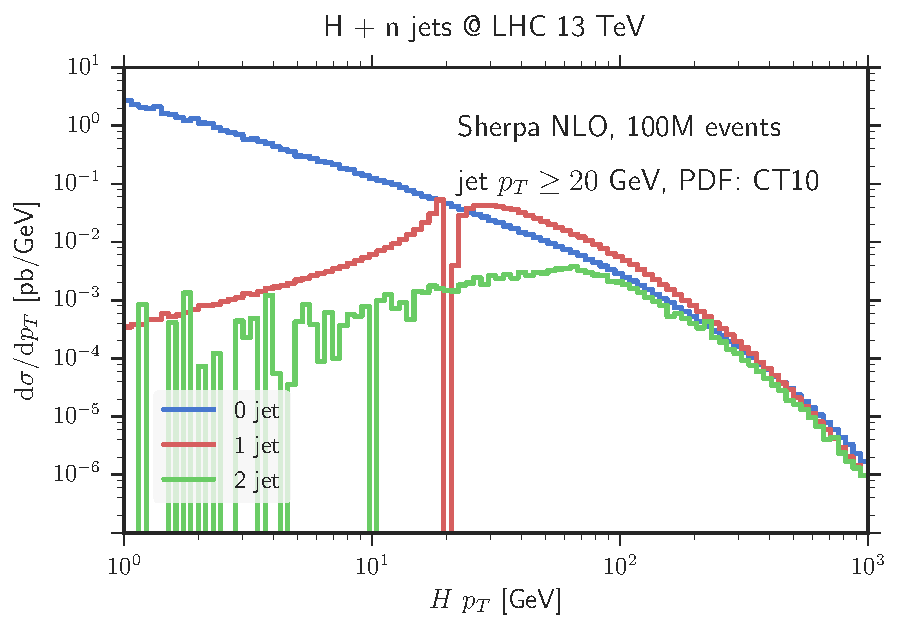
\includegraphics[width=\textwidth]{images/cmp100m_nlo_hpt.pdf}
\end{subfigure}
\hfill
\begin{subfigure}[]{0.49\textwidth}
	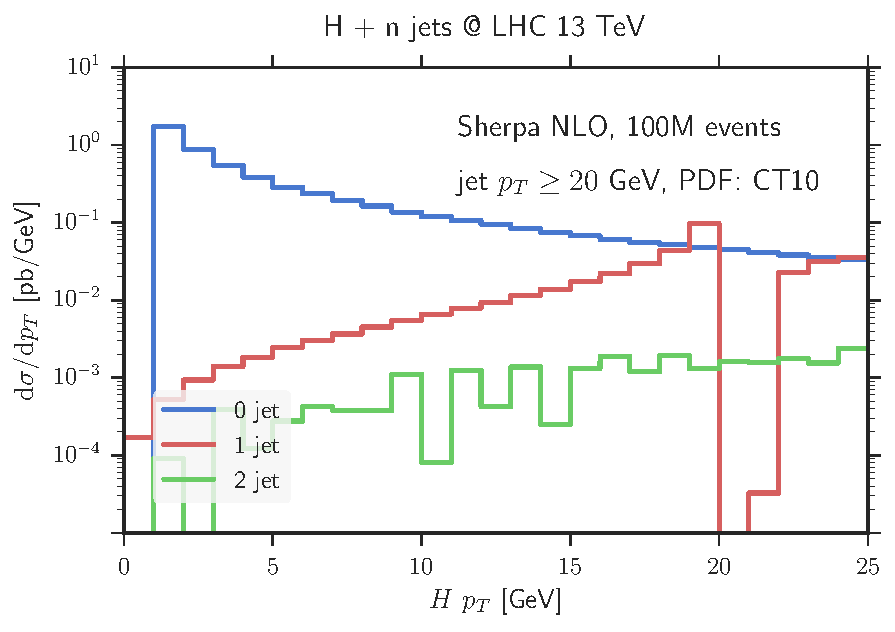
\includegraphics[width=\textwidth]{images/cmp100m_nlo_hptpeak.pdf}
\end{subfigure}
\caption{H pT NLO (0,1,2) jets}
%\label{fig:bla}
\end{figure}
%
\begin{figure}
\centering
\begin{subfigure}[]{0.49\textwidth}
	\includegraphics[width=\textwidth]{images/cmp100m_mcatnlo_hpt.pdf}
\end{subfigure}
\hfill
\begin{subfigure}[]{0.49\textwidth}
	\includegraphics[width=\textwidth]{images/cmp100m_mcatnlo_hptpeak.pdf}
\end{subfigure}
\caption{H pT MCatNLO (0,1,2) jets}
%\label{fig:bla}
\end{figure}
%


%
\begin{figure}
\centering
\begin{subfigure}[]{0.49\textwidth}
	\includegraphics[width=\textwidth]{images/scalesvar_band_hpt_10M.pdf}
	\caption{10M events}
\end{subfigure}
\hfill
\begin{subfigure}[]{0.49\textwidth}
	\includegraphics[width=\textwidth]{images/scalesvar_band_hpt_100M.pdf}
	\caption{100M events}
\end{subfigure}
\caption{Scale variations band}
%\label{fig:bla}
\end{figure}
%
\begin{figure}
\centering
\begin{subfigure}[]{0.49\textwidth}
	\includegraphics[width=\textwidth]{images/scalesvar_ratio_hpt_10M.pdf}
	\caption{10M events}
\end{subfigure}
\hfill
\begin{subfigure}[]{0.49\textwidth}
	\includegraphics[width=\textwidth]{images/scalesvar_ratio_hpt_100M.pdf}
	\caption{100M events}
\end{subfigure}
\caption{Scale variations ratio}
%\label{fig:bla}
\end{figure}
%
